\documentclass[10pt,a4paper]{article}
\usepackage[utf8]{inputenc}
\usepackage{amsmath}
\usepackage{amsfonts}
\usepackage{amssymb}
\usepackage{graphicx}
\usepackage{subcaption,graphicx}
\usepackage{listings}
\begin{document}
\textbf{Cap. 6 - 4 - } Para esta questão, os dados apresentados foram dispostos em um planilha com os meses sendo representados de $t = 0,...,14$ (planilha e script disponível no github[colocar o link aq dps]), além disso, foi utilizado o seguinte script em R para se obter as estimativas para os parâmetros e o valor para o coeficiente de determinação: \\

\begin{lstlisting}
	library(ggplot2)

	# Lê o conjunto de dados
	vendas <- read_excel ("vendas.xls")

	# Detalhes do ajuste de regressão linear para o problema
	vendas.lm <- lm(vendas ~ mês, data = vendas)
	summary(vendas.lm)
	
	# Ajuste do modelo aos dados 
	vendas.graph <- ggplot (vendas, aes(x = mês, y = vendas)) + geom_point()
	vendas.graph <- vendas.graph + geom_smooth(method="lm", col="black")
	vendas.graph
	
	# Ferramentas de diagnóstico
	plot (vendas.lm)
	plot (lm(vendas$vendas ~ vendas$mês), which = 4)
\end{lstlisting}

\textbf{a)} Para os dados apresentados, podemos descrever um modelo como sendo $y_t = \alpha + \beta t + e_t$ em que $t$ representa o mês, $y_t$ representa o faturamento da empresa no mês $t$, $\alpha$ representa o valor do faturamento no primeiro mês, $\beta$ equivale ao aumento do faturamento das empresas a cada mês e $e_t$ são erros aleatórios com média 0 e variância $\sigma^2$, além disso, é suposto que estes erros tenham uma distribuição normal e que os resíduos seguem a propriedade de  homocedasticidade. \\

\textbf{b)} por meio do comando lm(), utilizando o script apresentado anteriormente, pode-se estimar os parâmetros, com os erros padrões entre parênteses, como sendo $\hat{\alpha} = 0.718(0.284)$ e $\hat{\beta} = 0.405(0.034)$, assim, podemos dizer que no primeiro mês as empresas neste setor industrial apresentam um faturamento esperado de 0.72 e têm, em média, um crescimento de 0.41 no faturamento mensal. \\

\textbf{c)} Por meio do comando summary(vendas.lm) usado no script mostrado acima, obtemos um coeficiente de determinação igual a 0.91 e um coeficiente de determinação ajustado de 0.90, o que nos mostra que que obtivemos um bom ajuste para os dados utilizando este modelo. Como verificação adicional, construímos os seguintes gráficos gerados pelo comando lm():

\begin{figure}[ht]
    \centering
    \hspace*{-2.7cm}\begin{subfigure}{0.5\textwidth}
      \centering
      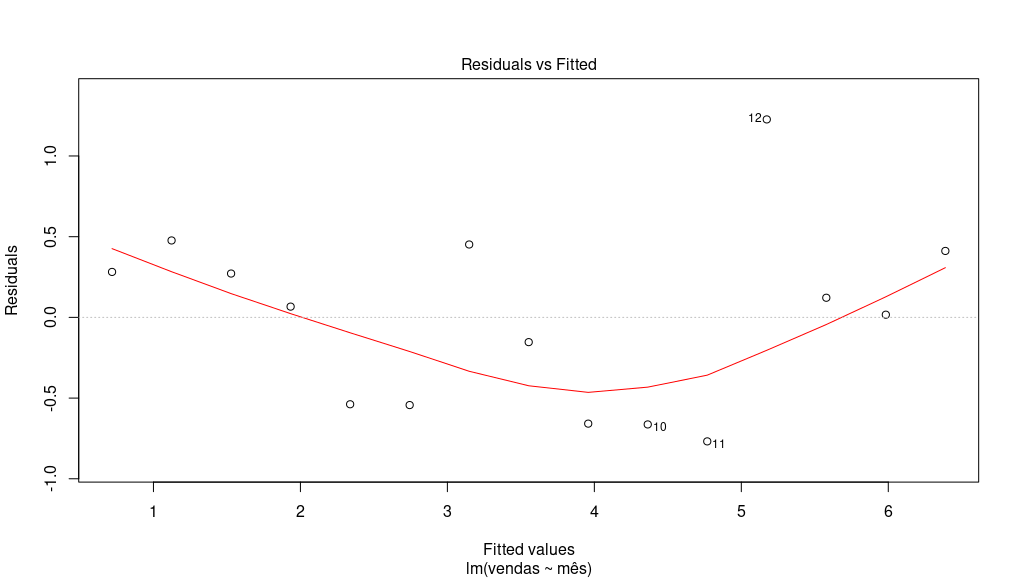
\includegraphics[width=9cm]{residualsFitted.png}
    \end{subfigure}%
    \hspace*{3cm}\begin{subfigure}{0.5\textwidth}
      \centering
      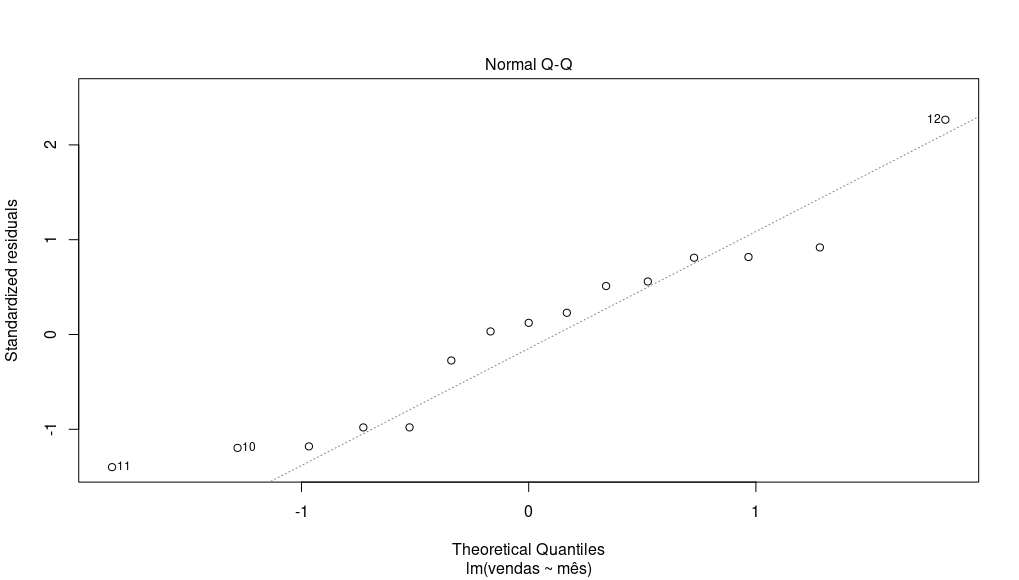
\includegraphics[width=9cm]{QQNormal.png}
    \end{subfigure}\\
    \hspace*{-2.7cm}\begin{subfigure}{0.5\textwidth}
      \centering
      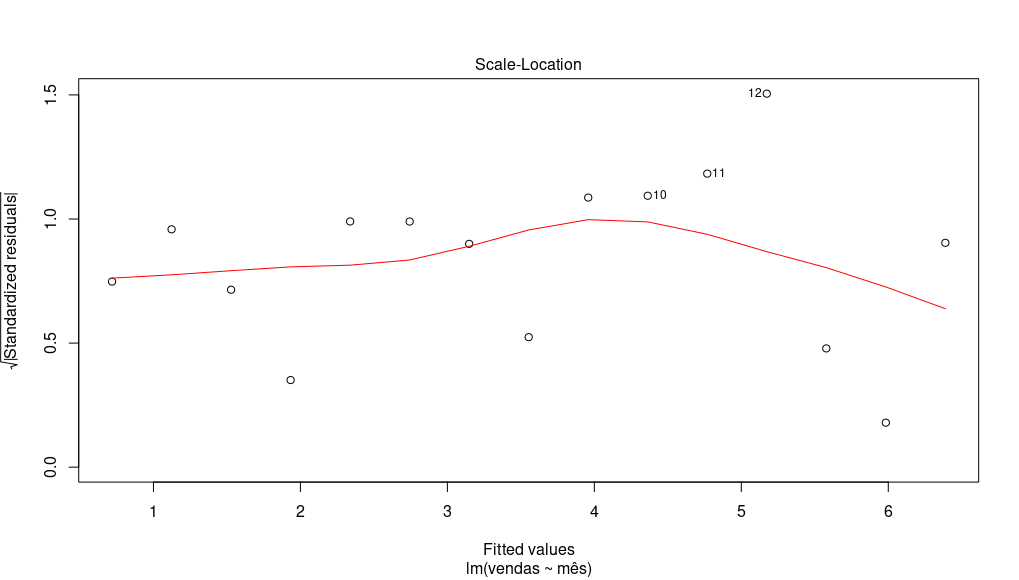
\includegraphics[width=9cm]{ScaleLocation.png}
    \end{subfigure}%
    \hspace*{3cm}\begin{subfigure}{0.5\textwidth}
      \centering
      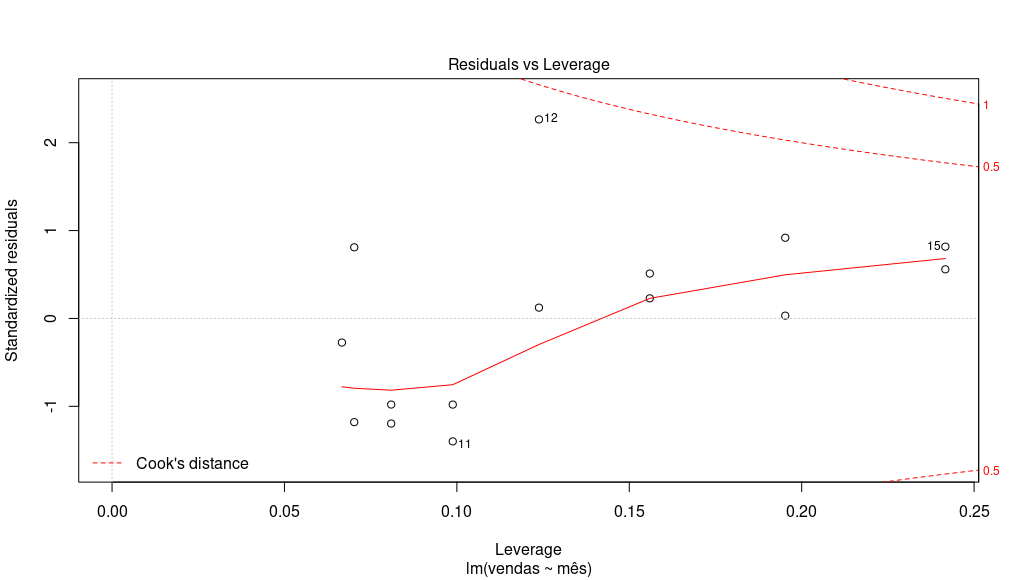
\includegraphics[width=9cm]{ResidualLeverage.png}
    \end{subfigure}
    \caption{Respectivamente gráficos de resíduos, QQ normal, Scale-Location e resíduos por alavancagem}
\end{figure}

A partir destas informações, podemos concluir que o ajuste do modelo foi razoável e concluindo que não há evidências contra as suposições de normalidade e de homocedasticidade.
\end{document}